\chapter{Evaluation}

\section{Theoretical evaluation}

The framework presented in this thesis has both advantages and disadvantages in design and implementation. The modular setup shown in Fig. \ref{fig:abstractoverview}, while providing easy extensibility, does require knowledge of the algorithms implemented therein. In contrary to LearnLib, where (from my experience) data structures are easily extended and onboarded to the learning, algorithm implementations are difficult to provide new solutions to, my framework allows extensibility on every front of it, with a steeper learning curve even with new input/output onboarding.

The framework, when implementing similar formalisms does require some redundancy, especially with the \emph{Learnable-LernableAdapter-Teacher} trio of implementation needed with new formalisms. The advantage of this sometimes redundant approach is the overall elimination of typecasting and uncertain genericity, allowing for exact application of methods and classes after bounding the generic parameters required, improving runtime, the compliance with object-oriented paradigms, and understandibility of an implementation without context of its abstrations. The \emph{Learnable} and \emph{Hypothesis} endpoints of input and output formalisms being interfaces provide flexibility by leveraging the multiple-inheritance (implementation) property of interfaces. This is used for example in the TTT implementation in order to extend upon classes of LearnLib, while still implementing my frameworks abstractions.

\subsection{Evaluation of DHC}

The Direct Hypothesis Construction algorithm, as theorized and proved in \cite{Steffen2011} and \cite{10.1007/978-3-642-34781-8_19}, terminates after at most $n^3mk+n^2k^2$ membership, and $n$ equivalence queries, where $n=|S|$, $k=|\Sigma|$ and m is the longest counterexample. The runtime complexity of these queries are difficult to evaluate, since they highly depend on implementation and context. Reaching the system under learning in the current implementation of input formalisms (String sequece or Mealy machine) takes no overhead, since the system behavior is stored in-memory. This might not be the case in other implementations, where the SUL might be reached through network communication or other such (non-negligible overhead) methods. In terms of membership queries, the current implementations differ. 

String sequences (\emph{StringSequenceLearnable}s) are stored in an input-output \emph{HashMap}, which allows $O(1)$ access assuming the values are evenly distributed in the buckets used by the hashing, worst-case scenario being $O(k)$. While access is fast, this method suffers in terms of space complexity, storing a numer of elements identical to $\mathcal{P}(\Sigma)\setminus\emptyset$, or in text, the powerset of $\Sigma$ without the empty set, resulting in a space complexity of $O(2^k)$.

The MealyMachine implementation (the \emph{MealyLearnable} class) provides a more reasonable $O(k)$ space complexity, but it struggles with runtime issues. The implementation, as discussed in the contribution section, provides ease of access to its data, with straightforward implementation of membership queries possible, not storing the automata in a graph-like format reduces efficiency. This results in a worst-case scenario of an $O(kt)$, where $t$ is the number of transitions of the automaton.

From the perspective of equivalence queries, the two implemented input formalisms both provide the same efficiency, since the implementation of this query is in the \emph{StringSequenceAdapter} class, both \emph{MealyLearnable} and \emph{StringSequenceLearnable} are queried using this implementation, which can be seen in Listing \ref{li:eqbruteforce}. This implementation is a brute-force way of proving equivalence of the hypothesis and the system under learning, operating by taking every permutation of every element in $\mathcal{P}(\Sigma)\setminus\emptyset$ and comparing outputs using membership queries for each of them. In order to mitigate some of this inefficiency, the implementation uses google guavas \emph{Sets.powerSet()} method, providing $O(k)$ space complexity as opposed to a brute-force $O(2^k)$ implementation. For each member of $\mathcal{P}(\Sigma)\setminus\emptyset$, the permutations are calculated using the \emph{Collections2.permutations()} method of guava, implementing the Johnson–Trotter algorithm. This results in a $O(2^kk!)$ number of membership queries considering the "worst case" of finding no counterexamples.

In summary, the best-case scenario of the current DHC implementation has an $O(n^3mk^2+n^2k^3+2^kk!k)$ runtime complexity, the worst case being $O(n^3mk^2t+n^2k^3t+2^kk!kt)$ depending on the variables presented above.

\subsection{Evaluation of TTT}

The TTT algorithm, as presented in \cite{10.1007/978-3-319-11164-3_26}, requires $O(n)$ equivalence queries and $O(kn^2+n\log m)$ membership queries, each of which takes $O(n+m)$ time, where $n=|S|$, $k=|\Sigma|$ and m is the longest counterexample. This is a very pessimistic estimate caused by the edge-case of a discriminator tree having $n$ height. The time complexity of the equivalence query implementation seen in \ref{li:eqbruteforce} still holds as $O(2^kk!)$, but is lengthened by the complexity of conversion between formalisms, being $O(nt)$ in the worst case, where t is the number of transitions of the current hypothesized automaton. Altogether, the worst case scenario has a $O((kn^2+n\log m)(n+m) + 2^kk!nt)$ time complexity. TTT also provides an efficient $\Theta(kn)$ space complexity\cite{10.1007/978-3-319-11164-3_26}.


\section{Experimental evaluation}

The experimental evaluation of the implemented algorithms were done using variations of the automaton seen in Fig. \ref{fig:dfaexamplemealyver}.a. This decision is based on the simplicity of extending the automaton accepting inputs containing $4i+3a$ to inputs containing $ni+(n-1)a$, where $n, i \in \mathbb{N}$. An example of this can be seen in Fig. \ref{fig:5ia}, where $n=5$. This solution is easily scalable and straightforward to implement even for large $n$s.

\begin{figure}
	\centering
	\begin{tikzpicture}[shorten >=1pt,node distance=3.5cm,on grid,auto] 
	\node[state,initial] (q_0)   {$q_0$}; 
	\node[state] (q_1) [right=of q_0] {$q_1$}; 
	\node[state] (q_2) [below=of q_0] {$q_2$}; 
	\node[state](q_3) [right=of q_2] {$q_3$};
	\node[state](q_4) [above right= 2.4cm of q_3] {$q_4$};
	\path[->] 
	(q_0) edge[]  node {a/$\top$} (q_1)
	edge [loop below] node {b/$\top$} ()
	(q_1) edge[]  node[pos=0.62]  {a/$\top$} (q_2)
	edge [loop below] node {b/$\top$} ()
	(q_2) edge[]  node [swap] {a/$\top$} (q_3) 
	edge [loop above] node {b/$\top$} ()
	(q_3) edge  node[pos=0.62] [swap] {a/$\bot$} (q_4)
	edge [loop above] node {b/$\top$} () 
	(q_4) edge[bend right=70]  node[pos=0.62] [swap] {a/$\top$} (q_0)
	edge [loop right] node {b/$\bot$} ();
	
	\end{tikzpicture}
	\caption{Example of an automaton accepting inputs containing $5i+4a$.}
	\label{fig:5ia}
\end{figure}

As seen in the theoretical evaluation, the size of the state space is not the only possible bottleneck, both algorithms (and the equivalence query implementation especially) slows with the size of the input alphabet. A simple solution of testing growing input alphabets using the Mealy machine seen in Fig. \ref{fig:dfaexamplemealyver}.a, is to add characters (transitions) without adding behavior. This does not end the minimal property of an automaton contrary to adding states without changing behavior, thus increasing runtime. An example of the described input alphabet extension can be seen in Figure \ref{fig:abcextended}.

\begin{figure}
	\centering
	\begin{tikzpicture}[shorten >=1pt,node distance=3.5cm,on grid,auto] 
	\node[state,initial] (q_0)   {$q_0$}; 
	\node[state] (q_1) [right=of q_0] {$q_1$}; 
	\node[state] (q_2) [below=of q_0] {$q_2$}; 
	\node[state](q_3) [right=of q_2] {$q_3$};
	\path[->] 
	(q_0) edge[]  node {a/$\top$} (q_1)
	edge [loop below] node {b/$\top$} ()
	edge [loop above] node {c/$\bot$} () 
	(q_1) edge[]  node[pos=0.62]  {a/$\top$} (q_2)
	edge [loop below] node {b/$\top$} ()
	edge [loop above] node {c/$\bot$} () 
	(q_2) edge[]  node [swap] {a/$\top$} (q_3) 
	edge [loop above] node {b/$\top$} ()
	edge [loop below] node {c/$\bot$} () 
	(q_3) edge  node[pos=0.62] [swap] {a/$\bot$} (q_0)
	edge [loop above] node {b/$\bot$} () 
	edge [loop below] node {c/$\bot$} () ;
	\end{tikzpicture}
	\caption{Example of the automaton seen in Fig. \ref{fig:dfaexamplemealyver}.a with an extended input alphabet $\Sigma=\{a, b, c\}$.}
	\label{fig:abcextended}
\end{figure}

After running the experiments, an obvious bottleneck could be found. The current brute-force equivalence query implementation is inefficient, as the theoretical evaluation suggested. Figure \ref{fig:stateruntime} shows the inefficiency observed when extending the states and the behavior of the learned automaton. The cause of this is the large number of states resulting in a large space of possibilities when brute-forcing equivalence, as theorized in the theoretical evaluation.

Figure \ref{fig:inputruntime} shows, that this is not the case with the extension of the input alphabet, since with the same number of sates, less future predictions are to be done, extending the input alphabet is not as taxing. In order to show (and compare) my implementation without this bottleneck, since these inefficiencies are not of the learning algorithms, but of the equivalence algorithm Fig. \ref{fig:inputruntime1} shows the exact same run as Figure \ref{fig:stateruntime} done with a near linear-time equivalence oracle implemented in LearnLib.

\begin{figure}
	\centering
	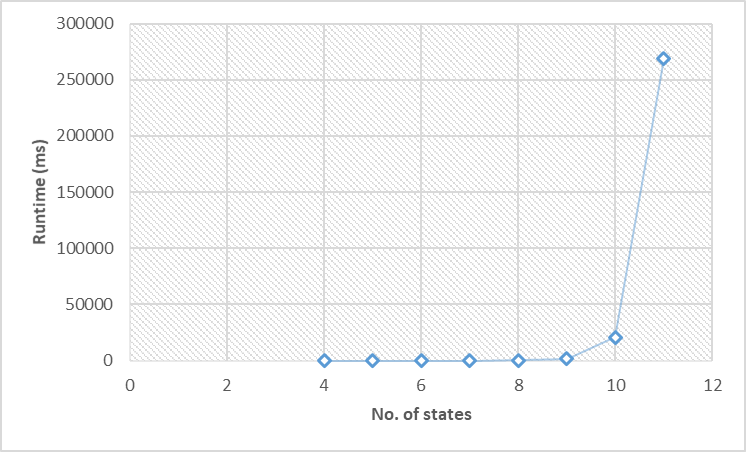
\includegraphics[width=0.7\linewidth]{figures/stateruntime}
	\caption{Figure showing the bottleneck the brute-force equivalence query implementation causes when increasing the state space.}
	\label{fig:stateruntime}
\end{figure}

\begin{figure}
	\centering
	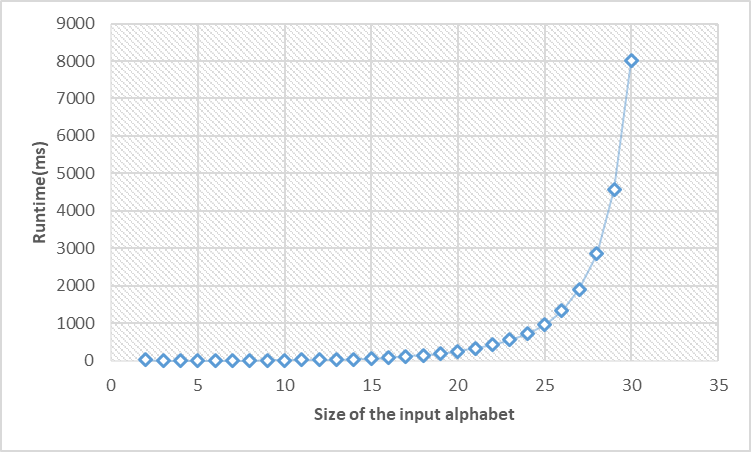
\includegraphics[width=0.7\linewidth]{figures/inputruntime}
	\caption{Figure of the runtime observed when the input alphabet was increased without any behavioral change.}
	\label{fig:inputruntime}
\end{figure}



\begin{figure}
	\centering
	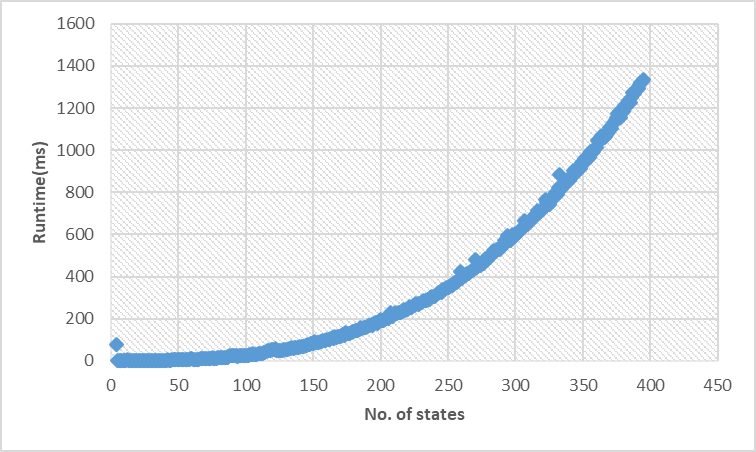
\includegraphics[width=0.7\linewidth]{figures/inputruntime1}
	\caption{Run after clearing up the bottleneck by using a near linear runtime equivalence checking algorithm implemented in LearnLib.}
	\label{fig:inputruntime1}
\end{figure}
